\label{section:etl}
In this chapter we will describe the process used for extracting, transforming and loading data into the Data Warehouse.

I analyzed the multiple problems encountered during the ETL development as well as the process employed by Reply.
Most problems were however solved by Axpo specialists, since their specific knowledge was required.

I also asked Reply to keep track of all the issues encountered as well as their status.

This can be used both by Reply, to better organize its work, and by Axpo, to understand if a delay is due to an unexpected issue and how well Reply is performing.

The resulting document can be used both as a small layer of documentation and to produce some tests for the more vulnerable parts of the ETL processes.

\section{ETL Operations}
    This section will provide a description of the main operations performed by the ETL process.
An exhaustive list is not provided, since describing each operation of them would be extremely long and repetitive.

\subsection{Extraction}
    Most processes are executed daily, so the downloaders usually retrieve files only for the current day.
    However the downloaders can also be easily configured to retrieve a range of dates, in case of history retrieval (which is only used to initialize the Data Warehouse).
    
    Each downloaded file is saved to the \texttt{rawdata} folder on DataLake \textit{as-is}.
    
    \subsubsection{Provider types} \label{section:etl:provider_types}
        Different download techniques are used, depending on the kind of services exposed by a particular provider.
        
        \paragraph{FTP}
            Several providers provide an FTP share, where they upload a few files each day, which contain the data for that given day.
            
            In this case the downloader just needs to connect to the FTP server and retrieve the files.
            
            Files stored here are usually either in \texttt{csv}, \texttt{xml} or \texttt{xls} format.
            
        \paragraph{API}
            Other websites provide an API which can be queried for data.
            
            The resulting datasets are usually in \texttt{json} or \texttt{xml} format.
            
            In this case the downloader makes several calls to the API, each one with different parameters.
            
        \paragraph{SQL databases}
            These providers provide the easiest interface, since it is possible to directly perform queries and extract the data in nearly any format.
            
            Since most of these providers are internal services owned by Axpo, their number is limited, compared to all the public providers.
            
        \paragraph{Web scraping}
            Some websites do not expose their data through any particular service.
            
            In this case the only solution is to build a web scraper, which simulates human web navigation retrieving information manually.
            
            This approach is the most complex and time consuming, since it has to be build \textit{ad hoc} for the website.
            Moreover, its re-usability across different websites is low, if non-existent, so it needs to be developed each time from scratch.
        
\subsection{Transformation}
    Databricks retrieves the files saved on \texttt{rawdata} and performs some operations on them, before saving the resulting datasets in \texttt{.csv} format on the \texttt{srcdata} folder in DataLake.
    
    The most commonly executed operations are:
        \begin{itemize}
            \item Reading the dataset: depending on its format different methods are needed
            \item Renaming columns
            \item Dropping unneeded columns
            \item Appending the file download date to each row, where not already present
            \item Unpivoting the dataset, if needed
            \item Normalizing column names
        \end{itemize}
        
    \paragraph{Unpivoting}
        A consistent number of datasets provide a value for each hour in a day in an apposite column.
        
        It is necessary to change the format, displaying on one column the hour and in another one the value.
        This operation is called \textit{unpivoting} or \textit{melting}.
        
        \begin{table}
            \centering
            \begin{tabular}{|c|c c c c c|}
                \toprule
                 Zone  & H1 & H2 & H3 & ... & H25   \\
                 \midrule
                 North & 12 & 15 & 14 & ... & 0     \\
                 South & 32 & 29 & 28 & ... & 0     \\
                 \bottomrule
            \end{tabular}
            \quad
            \begin{tabular}{|c|c c|}
                \toprule
                 Zone  & Hour  & Value   \\
                 \midrule
                 North & H1    & 12     \\
                 North & H2    & 15     \\
                 North & H3    & 14     \\
                 North & ...   & ...    \\
                 North & H25   & 0      \\
                 South & H1    & 32     \\
                 South & H2    & 29     \\
                 South & H3    & 28     \\
                 South & ...   & ...    \\
                 South & H25   & 0      \\
                 \bottomrule
            \end{tabular}
            \caption{Normal (left) and unpivoted (right) tables.}
            \label{tab:etl:melt}
        \end{table}
        
        Table \ref{tab:etl:melt} provides an example of unpivoting.
        In the left table we have 26 columns, one representing the zone and a column for each hour\footnote{There are 25 hours to account for DST.}, while in the right table we have 3 columns: zone, hour and value.
    
    \paragraph{Column names normalization}
        Some columns do not respect the naming convention decided for the Data Warehouse.
        
        Some columns may contain special characters or spaces, which cause problems when inserted into a database table.
        
        Several operations are performed to remove or replace these characters.
        
        For example, spaces and dashes are replaced with an underscore, parentheses of any type are removed and the character \code{\&} is replaced with its literal representation \code{and}. \\
        Also, all names are converted into lowercase.
            
\subsection{Loading}
    Databricks retrieves the files from \texttt{srcdata} and loads the data onto the Data Warehouse.
    
    The Data Warehouse, through several tables, views and procedures, performs some final operations on the data, before appending the new values onto the final tables.
    
    \subsubsection{Data Warehouse procedures}
        The Data Warehouse contains three schemas:
            \begin{itemize}
                \item \texttt{src} \textit{(source)}
                \item \texttt{stg} \textit{(staging)}
                \item \texttt{dm}  \textit{(data mart)}
            \end{itemize}
        
        \paragraph{\textit{Source} schema}    
            Databricks loads the data directly into the \texttt{src} schema tables, without performing any operations in it.
            
            This schema contains a table for each flow, with the same structure as the \texttt{csv} file.
            All values loaded in these tables are initially represented as strings but they are then casted to their actual data type through apposite views.
            
            These views are still located in the same schema, and there is a view for each table.
            
            Each time new data are inserted into those tables, the old values are erased.
        
        \paragraph{\textit{Staging} schema}
            Through some stored procedures, the views present in the \texttt{src} schema are read and some additional operations are applied on the data.
            
            The result is then saved on some apposite tables stored under the \texttt{stg} schema.
            
            As with the \texttt{src} schema, when inserting into these tables, the previously existing data are erased.
            
            The most significative differences between the two schemas are the structure and the amount of tables.
            
            In the \texttt{src} schema, there are as many tables as flows and their structure is identical to the \texttt{csv} files stored on DataLake.
            
            The tables on the \texttt{stg} schema are, on the other hand, much less and resemble the structure of the final tables.
            Moreover, flows from different providers are stored together in these tables.
            
            The operations performed by the stored procedures are in charge of changing the data structure, from the one used in the \texttt{csv} to the one needed by the final tables, and to add some constants: for example, if we have a \texttt{src} table containing information about \textit{MSD}, its provider will surely be \textit{GME}\footnote{
                \textit{MSD} information are only provided by \textit{GME}.
                For more details, see appendix \ref{section:providers:gme}.
            }.
            
        \paragraph{\textit{Data Mart} schema}
            This schema contains the final tables, which will be queried by the end-users.
            
            Through apposite stored procedures, the content of the \texttt{stg} tables are appended into the \texttt{dm} tables.
            
            These procedures pay special attention to checking if the values to be inserted are already present in the Data Warehouse and, if they are, they do not perform any action.
            
            This has been done to prevent duplicate data, which may be created by running more than once the ETL process (which may happen in case of errors).
            
    \subsubsection{Logging} \label{section:etl:logging}
        All loading operations are traced to a log table, which is analyzed in case of alerts to understand when and how a process failed.
        
        \paragraph{Logging}
            Logging is performed by invoking several stored procedures on the Data Warehouse, which write information to apposite tables.
            These information contain:
                \begin{itemize}
                    \item The id of the process
                    \item The provider name
                    \item The data stream name for that given provider
                    \item Two timestamps, for insertion and update respectively
                    \item Some flags to indicate the operations already performed on the data
                \end{itemize}
            
            Logs are written during each phase of the ETL process for each flow.
        
        \paragraph{Alerts}
            Alerts are generated by a monitoring system set in Databricks.
            Jobs can be set to send mails when a jobs starts, ends or fails.
            
            Upon job failure, Databricks sends a mail to specific users.
            The mail contains a link to the cell which raised an error, along with the id of the process which failed.
            
            It is possible both to analyze the code and to query the database logging tables (using the id contained in the mail) to retrieve additional information.
        
        \paragraph{Monitoring tools}
            Currently there are no tools actively monitoring the quality of the data present in the Data Warehouse apart from the alert system.
            
            This is done under the assumption that if the data are inserted into the Data Warehouse they are already of acceptable quality.
            However, if some errors happen to elude the monitoring system, there is not currently any way to notice the problem.
    
\section{Issues} \label{section:etl:difficulties}
    During development of the ETL process, there have been many difficulties.
This section will list the most relevant problems encountered.

\subsection{File Encoding}
    This problem is related mainly to \texttt{csv} files.
    Most files are encoded in \texttt{ANSI} format, but a few providers used special characters which required a different encoding.
    
    For example, some energy plants or technical description contain accented characters, which are not supported by the \texttt{ANSI} format.
    
    Spotting this kind of problems isn't easy, since not all files may present special characters.
    
    The solution, on the other hand is easy, since it is sufficient to use \texttt{utf-8} encoding.

\subsection{Wrong File Extension}
    We also encountered an issue related to a wrong file extension.
    Terna exposes its data in Excel format, but the websites presents a low level of consistency in its files.
    
    While most files were in \texttt{xls} format, a few were in \texttt{xlsx} format, which requires a different method for reading it.
    However, upon further analysis, the files proved to be regular \texttt{xls} with a wrong file extension.
    As a result, extensions are ignored when reading files.
    
% \subsection{DST} \label{etl:problems:dst}
%     One of the problems most commonly encountered is that of Daylight Saving Time (DST).
    
%     On the last Sunday of March, time is shifted one hour forward at 2am while, on the last Sunday of October, time is shifted one hour back at 3am.
    
%     As a consequence, in March we have a day with 23 hours, since the hour between 2 and 3am is skipped, while in October we have a day with 25 hours, since the hour between 2 and 3am is repeated twice.
    
%     The main problem is that each provider handles these hours in their own way, using their own notation.
%     As a consequence, the same value may have different meanings depending on the provider.
    
%     This issue was 

% \subsection{Gas day} \label{etl:problems:gasday}
%     \todoetl{gas day}
%     gas day goes from 6am to 6am.
%     however dst changes are handled differently: gas days have always 24 hours, which means that during dst each day is shifted by one hour. (6-6, 7-7)
% \subsection{Timezones}
%     \todoetl{timezones}
%     some sites provide dates in local time, which means that they must be normalized
    
%     in some cases we have both the problem of timezones and that of dst
    
%     Cambio ora e.g. londra avviene tra 1/2, noi tra 2/3 (che poi e` lo stesso momento, vedi fuso orario)

\subsection{Aggregation/Deaggregation} \label{etl:problems:aggregation_deaggregation}
    Some providers offer data with granularity different from the needs of Axpo users.
    
    In this case it is necessary to either aggregate or deaggregate the data downloaded, before inserting it into the Data Warehouse.
    
    These processes present their own difficulties however.
    
    \paragraph{Aggregation}
        The difficulty in aggregating is understanding which operation is more appropriate for each kind of data.
        
        Let's assume we want to aggregate into hourly data information provided every 15 minutes.
        
        Energy consumptions\footnote{
            Energy consumption refers to the amount of electricity used in a given time range, expressed in MW.
        }, for example, need to be summed, while temperature forecasts need to be averaged, since it would make no sense to sum them.
        
    \paragraph{Deaggregation}
        Splitting aggregated data into a finer granularity presents additional problem to those of aggregating.
        
        For example, let's assume we want to know the hourly energy consumption for a given user.
        If we have a single value for the whole day, it is not reasonable to divide that value by 24, since it is very unlikely the consumption has been constant during the whole day.
        
        In this case the correct operation is infer a consumption model from other available data and to assume this user will behave similarly.
        Then the total value will be divided proportionately to the model.
        
        This is however a specific example, in general it is impossible to give a rule of thumb, since each case presents different properties and must be analyzed individually.
        
    \paragraph{Time shifts and time formats}
        Choosing the correct operation is not the only problem however.
        
        Different time formats, such as gas day, and time shifts, caused by DST, make these operations even more complex.
        
        The first 6 hours (\textit{0-6am}) of a ``standard'' day are part of the previous gas day.
        However, during DST, these hours become 7 (\textit{0-7am}), since gas days always have 24 hours, while standard days can have 23, 24 or 25 hours\footnote{
            For more details, see sections \ref{section:dwh:gas_day} (Gas day) and \ref{section:dwh:dst} (DST).
        }.
        
        In these cases more complex queries are required to obtain the correct data before applying aggregation or deaggregation operations.
    
\subsection{Different Update Frequencies}
    Each provider updates data with its own frequency.
    
    Update frequencies vary greatly, ranging from hourly to monthly updates.
    There are also some particular scenarios, for example a certain provider updates its data on Monday, either Tuesday or Wednesday (with no apparent discerning factors) and Friday.
    
    This causes issues when scheduling jobs, since it is necessary to schedule each job independently.
    \begin{table}
        \centering
        \begin{tabular}{|l|l|}
            \toprule
            Session          & Scheduled Start           \\
            \midrule
            Daily A          & 0 30 13,14 ? * * *        \\
            Daily B          & 0 30 8 * * ?              \\
            Daily C          & 0 10 18 ? * * *           \\
            Daily D          & 0 30 8,17 ? * * *         \\
            Daily E          & 0 30 11 1,2,3,4,5 * ? *   \\
            Intra-daily 1    & 0 30 15 ? * * *           \\
            Intra-daily 2    & 0 0 17 ? * * *            \\
            Intra-daily 3    & 0 30 8 ? * * *            \\
            ...              & ...                       \\
             \bottomrule
        \end{tabular}
        \caption{Jobs scheduled for a specific provider.}
        \label{tab:gme_job_schedules}
    \end{table}
    
    Table \ref{tab:gme_job_schedules} shows an example of jobs scheduled for a specific website providing market data.
    All the start times are in \textit{crontab} notation\footnote{
        The values indicate respectively seconds, minutes, hours, day of month, month, day of week and year.
        For more information about \textit{crontab} notation, see \cite{bib:crontab:notation}.
    }.
    
    Each one of these jobs executes multiple Databricks notebooks, each one downloading a specific data stream.

\section{Examples}
    In this section we will list a few examples to give a more hands-on idea of some of the problems encountered during development.
    
    \subsection{CSV Parsing}
        Reading from a \texttt{csv} file is not always a trivial operation.

Several files contain some heading lines with additional information.
When reading these files it is necessary to apply additional operations to extract these information.

For example, a certain provider exposes market information in different files.
Depending on the file, different operations must be applied.

\paragraph{First rows metadata}
    \begin{figure}
        \centering
        \fbox{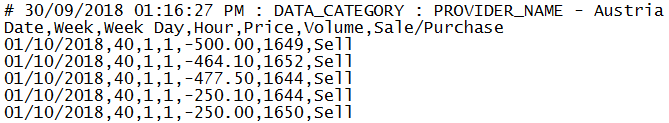
\includegraphics[width=.75\textwidth]{res/etl/epex_ac.PNG}}
        \caption{Metadata in first rows of a \texttt{csv} file.}
        \label{fig:etl:csv:ac}
    \end{figure}
    
    As we can see from Figure \ref{fig:etl:csv:ac}, the first row of the \texttt{csv} file requires special attention.
    
    From it we can extract information about\footnote{
        Some information are under a non-disclosure clause and as such have been anonymized.
    }:
        \begin{itemize}
            \item Creation date \textit{(30/09/2018 01:16:27 PM)}
            \item Category \textit{(DATA\_CATEGORY)}
            \item Provider \textit{(PROVIDER\_NAME)}
            \item Country \textit{(Austria)}
        \end{itemize}
    These information are then appended to each row of the dataset and stored on the Data Warehouse.

\paragraph{Multiple data formats}
    \begin{figure}
        \centering
        \fbox{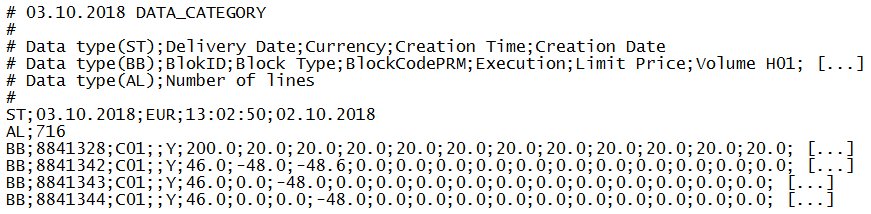
\includegraphics[width=\textwidth]{res/etl/epex_bb.png}}
        \caption{\texttt{Csv} with multiple data formats.}
        \label{fig:etl:csv:bb}
    \end{figure}
    
    For a different data stream, the first 6 rows of the file define some metadata of the dataset, and need to be treated separately.
    Figure \ref{fig:etl:csv:bb} shows the format of the data.
    
    This file contains three different types of data, each with its own format and structure.
    The first rows define the columns available for different types of data.
    The first column of the dataset specifies the data type.
    
    As we can see from Figure \ref{fig:etl:csv:bb}, the first three rows (of type, respectively, \texttt{ST}, \texttt{AL} and \texttt{BB}) have a different number of columns.
    This causes problems when reading the dataset, and requires splitting the file in three datasets, each for a data type.
    
    The first line is, instead, handled similarly to the situation described in the previous example.
    \subsection{Unpredictable File Names} \label{section:etl:terna}
        The website of Terna S.p.A.\footnote{
    Terna S.p.A. is the most important Transmission System Operator in Italy.
    It manages almost all of the Italian energy transmission grid.
} is an example of technical problems which heavily influenced the extraction process.

\paragraph{Premise}
    Terna provides each day an Excel file containing several data.
    An intuitive approach would be to download directly these files.
    
    However, due to the inconsistencies described in the next paragraph, it became necessary to navigate the website with a web scraper, which is far more complex to develop than a simple downloader.
    
\paragraph{Inconsistencies}
    The main problem with the Terna website is that there isn't any naming convention for the Excel files.
    
    As we can see from Table \ref{tab:etl:terna:files}, files related the same data category for consecutive days have both very different names and different extensions.
    Moreover, some files marked as \texttt{.xlsx} are actually just \texttt{.xls} with a wrong file extension.
    
    \begin{table}
        \centering
        \begin{tabular}{|c c c|}
            \toprule
            Date & Filename & Extension \\
            \midrule
            11/04/2019 & 73 & XLS  \\
            10/04/2019 & 52 & XLSX \\
            09/04/2019 & 31 & XLS  \\
            08/04/2019 & 03 & XLS  \\
            \bottomrule
        \end{tabular}
        \caption{
            Filenames and extensions for files downloaded from \texttt{Terna.it}.
            All files are related to the same category.
        }
        \label{tab:etl:terna:files}
    \end{table}
    
  \paragraph{Web scraper}
    Since it is impossible to predict which files to download, the only possible approach is to navigate the website and download the files manually or through a web scraper.
    The downloader uses Selenium to navigate and interact with Terna website, and to retrieves the URLs of several \texttt{.xls} and \texttt{.xlsx} files, which will be downloaded by Databricks.
    
    This process is by far slower than a normal downloader, but allows us to bypass the filename issue.
    \subsection{Website Navigation}
        Damas\footnote{
    Damas is a private web portal managed by Terna S.p.A.
    It provides data related to energy transfers between Italy and bordering countries.
    Information from this website are private, meaning that each company can only see their own energy transfers.
} is an example of a website which requires complex navigation logic.

The website offers a simple interface for selecting a time range and showing the data for that given range.
However, this system presents two limitations.

\paragraph{Limited date range}
    First of all, the maximum date range allowed is 31 days.
    If a user tries to perform a query on a bigger date range, the system shows an error message.
    
    This means that it is necessary to perform 12 queries to download a whole year.

\paragraph{No DST}
    The other problem is that if a date range contains a DST change, the website shows the following error message:

    \begin{center}
        \texttt{
            One of the days in the interval BUSDAY(30.03.2019) and\\ BUSDAYTILL(31.03.2019) contains clock change days.
        }
    \end{center}
    
    As shown by the message, it is impossible to download even a small amount of days, if a DST change occurs between them.

    The solution would be to download these dates individually, while downloading the rest of the data in ranges smaller than 31 days.
    However, since each year has different dates for DST changes, it would be necessary to set up these date manually for each year in the downloader.
    
    In the end, the best solution, even though it's computationally less effective, is to download each day individually.
    In this way there is no need to group dates into ranges and to pay attention to DST changes.
    The download process, on the other hand, is slower than downloading data in a batch.
    